\section{Evaluation}\label{sec:eval}

\begin{table*}
  \centering
  \caption{The analysis precision of $\tool$ without refinement
  (\stextsf{no-refine}), with refinement (\stextsf{refine}), and their
  difference ($\Delta$)}
  \label{table:precision}
  \resizebox{\textwidth}{!}{%
  \begin{tabular}{c|c?c|c?c|c?c|c}
    \multirow{2}{*}{\textbf{Checker}} &
    \multirow{2}{*}{\textbf{Bug Kind}} &
    \multicolumn{6}{c}{
      \textbf{Precision = (\# True Bugs) / (\# Detected Bugs)}
    }\\\cline{3-8} &&
    \multicolumn{2}{c?}{no-refine} &
    \multicolumn{2}{c?}{refine} &
    \multicolumn{2}{c}{$\Delta$}\\

    \specialrule{.1em}{.0em}{.0em}

    \myrowc{2}
    {Reference}     {60 / 116 (51.7\%)} {60 / 116 (51.7\%)} {\md{12}{3}{51.7}}
    {UnknownVar}    {17 / 72 (23.6\%)}  {17 / 72 (23.6\%)}  {\md{12}{3}{51.7}}
    \myrowh
    {DuplicatedVar} {43 / 44 (97.7\%)}  {43 / 44 (97.7\%)}  {\md{12}{3}{51.7}}

    \hline

    \myrowc{1}
    {Arity}         {60 / 116 (51.7\%)} {60 / 116 (51.7\%)} {\md{12}{3}{51.7}}
    {MissParam}     {17 / 72 (23.6\%)}  {17 / 72 (23.6\%)}  {\md{12}{3}{51.7}}

    \hline

    \myrowc{1}
    {Assertion}     {60 / 116 (51.7\%)} {60 / 116 (51.7\%)} {\md{12}{3}{51.7}}
    {Assertion}     {17 / 72 (23.6\%)}  {17 / 72 (23.6\%)}  {\md{12}{3}{51.7}}

    \hline

    \myrowc{2}
    {Operand}       {60 / 116 (51.7\%)} {60 / 116 (51.7\%)} {\md{12}{3}{51.7}}
    {NoNumber}      {17 / 72 (23.6\%)}  {17 / 72 (23.6\%)}  {\md{12}{3}{51.7}}
    \myrowh
    {Abrupt}        {43 / 44 (97.7\%)}  {43 / 44 (97.7\%)}  {\md{12}{3}{51.7}}

    \specialrule{.1em}{.0em}{.0em}

    \mysrowh
    {\textbf{Total}}{43 / 44 (97.7\%)}  {43 / 44 (97.7\%)}  {\md{12}{3}{51.7}}

  \end{tabular}
  }
  \vspace*{-1.5em}
\end{table*}

We implemented $\tool$ as an open-source tool~\footnote{The link is anonymized
because of a double-blind review process} in Scala by extending $\jiset$, a
JavaScript IR-based semantics extraction toolchain, with a worklist-based
fixpoint algorithm for type analysis.  Since $\jiset$ cannot automatically
compiles algorithm steps written in an uncommon writing style to $\ires$
instructions, our tool only reports type-related specification bugs detected in
fully compiled abstract algorithms.  For built-in libraries, we only targeted
abstract algorithms of essential built-in objects: \jscode{Array},
\jscode{Object}, \jscode{Function}, \jscode{Math}, \jscode{Proxy}, and objects
for primitive types.

To evaluate $\tool$, we answer the following research questions:
\begin{itemize}
  \item RQ1. \textbf{(Performance)} How long does $\tool$ take to perform type
    analysis for JavaScript specifications?
  \item RQ2. \textbf{(Precision)} How many type-related specification bugs
    detcted by $\tool$ are true bugs?
  \item RQ3. \textbf{(Effect of Refinement)} Does the condition-based refinement
    improve the analysis precision with endurable performance degradation?
  \item RQ4: \textbf{(Detection of New Bugs)} Does $\tool$ detect new
    specification bugs in the latest version of ECMAScript?
\end{itemize}
The draft of the next version of ECMAScript (ES12, 2021) is fixed on March 9,
2021.  Thus, we targeted all different 864 versions existed in the official
ECMAScript repository~\footnote{https://github.com/tc39/ecma262} for the recent
three years from January 1, 2018 to March 9, 2021.  We performed our experiments
on five Ubuntu machines equipped with 4.2GHz Quad-Core Intel Core i7 and 32GB of
RAM.


\subsection{Performance}\label{sec:performance}

Figure~\ref{fig:stat} shows four statistics of type analysis using $\tool$ for
864 versions of ECMAScript: (a) the number of analyzed functions, (b) the number
of flow- and type-sensitive views, (c) the number of worklist iterations, and
(d) the analysis time.  For each version of ECMAScript, \inred{1,999.9}
functions (\stextsf{func}) are analyzed and \inred{1,999.9} functions among them
are fully compiled (\stextsf{full-func}) on average.  Since the compile rules in
$\jiset$ is more suitable for recent versions, the number of fully compiled
functions in older versions are less than in more recent versions.  $\tool$
keeps different abstract environments for each functions divided by flow- and
type-sensitive views.  In the analysis result, \inred{1.3}M views existed for
each version and \inred{1.3}K views existed for each function on average.

We measured performance of $\tool$ based on the number of iterations for
worklist algorithm and the analysis time.  For each version of ECMAScript,
$\tool$ took \inred{300.0} seconds with \inred{19,999.9} iterations of worklist
algorithm on average.  The analysis time consists of \inred{10.0} seconds for
the specification extraction (\stextsf{extract} with gray bars), \inred{340.0}
seconds for the type analysis (\stextsf{analyze} with blue bars), \inred{10.0}
seconds for the bug detection (\stextsf{detect} with red bars).


\subsection{Precision}\label{sec:precision}

\begin{table}
  \centering
  \caption{The creators and resolvers of true bugs.}
  \label{table:author}
  \resizebox{\columnwidth}{!}{%
  \begin{tabular}{c|c|c?c|c|c}
    \multicolumn{3}{c?}{\textbf{Creator}} &
    \multicolumn{3}{c}{\textbf{Resolver}}\\\hline

    \textbf{Committee} &
    \textbf{Outsider} &
    \textbf{Inherited} &
    \textbf{Committee} &
    \textbf{Outsider} &
    \textbf{NotYet}\\\hline

    \inred{60} &
    \inred{12} &
    \inred{20} &
    \inred{60} &
    \inred{23} &
    \inred{10}\\
  \end{tabular}
  }
  \vspace*{-1.5em}
\end{table}

\begin{figure}
  \centering
  \begin{subfigure}[b]{0.24\textwidth}
    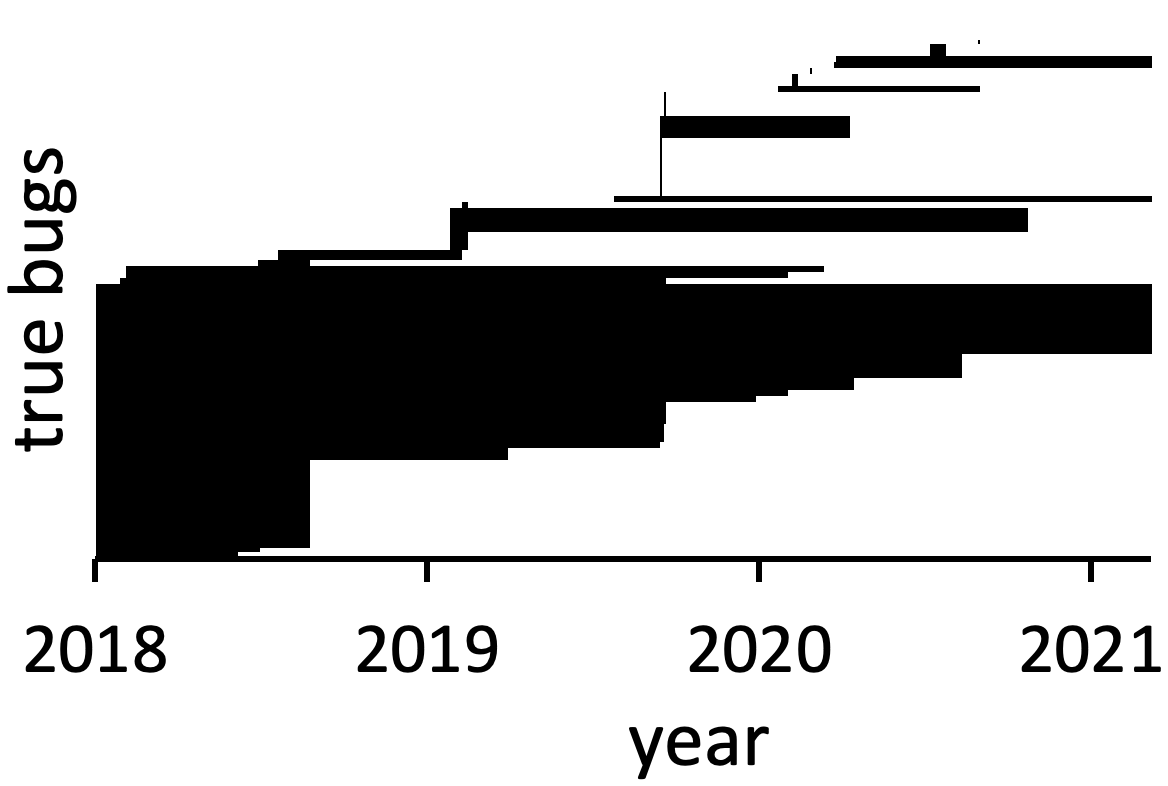
\includegraphics[width=\textwidth]{img/ttl-chro}
    \caption{Existence period sorted by creation time.}
  \end{subfigure}
  \begin{subfigure}[b]{0.24\textwidth}
    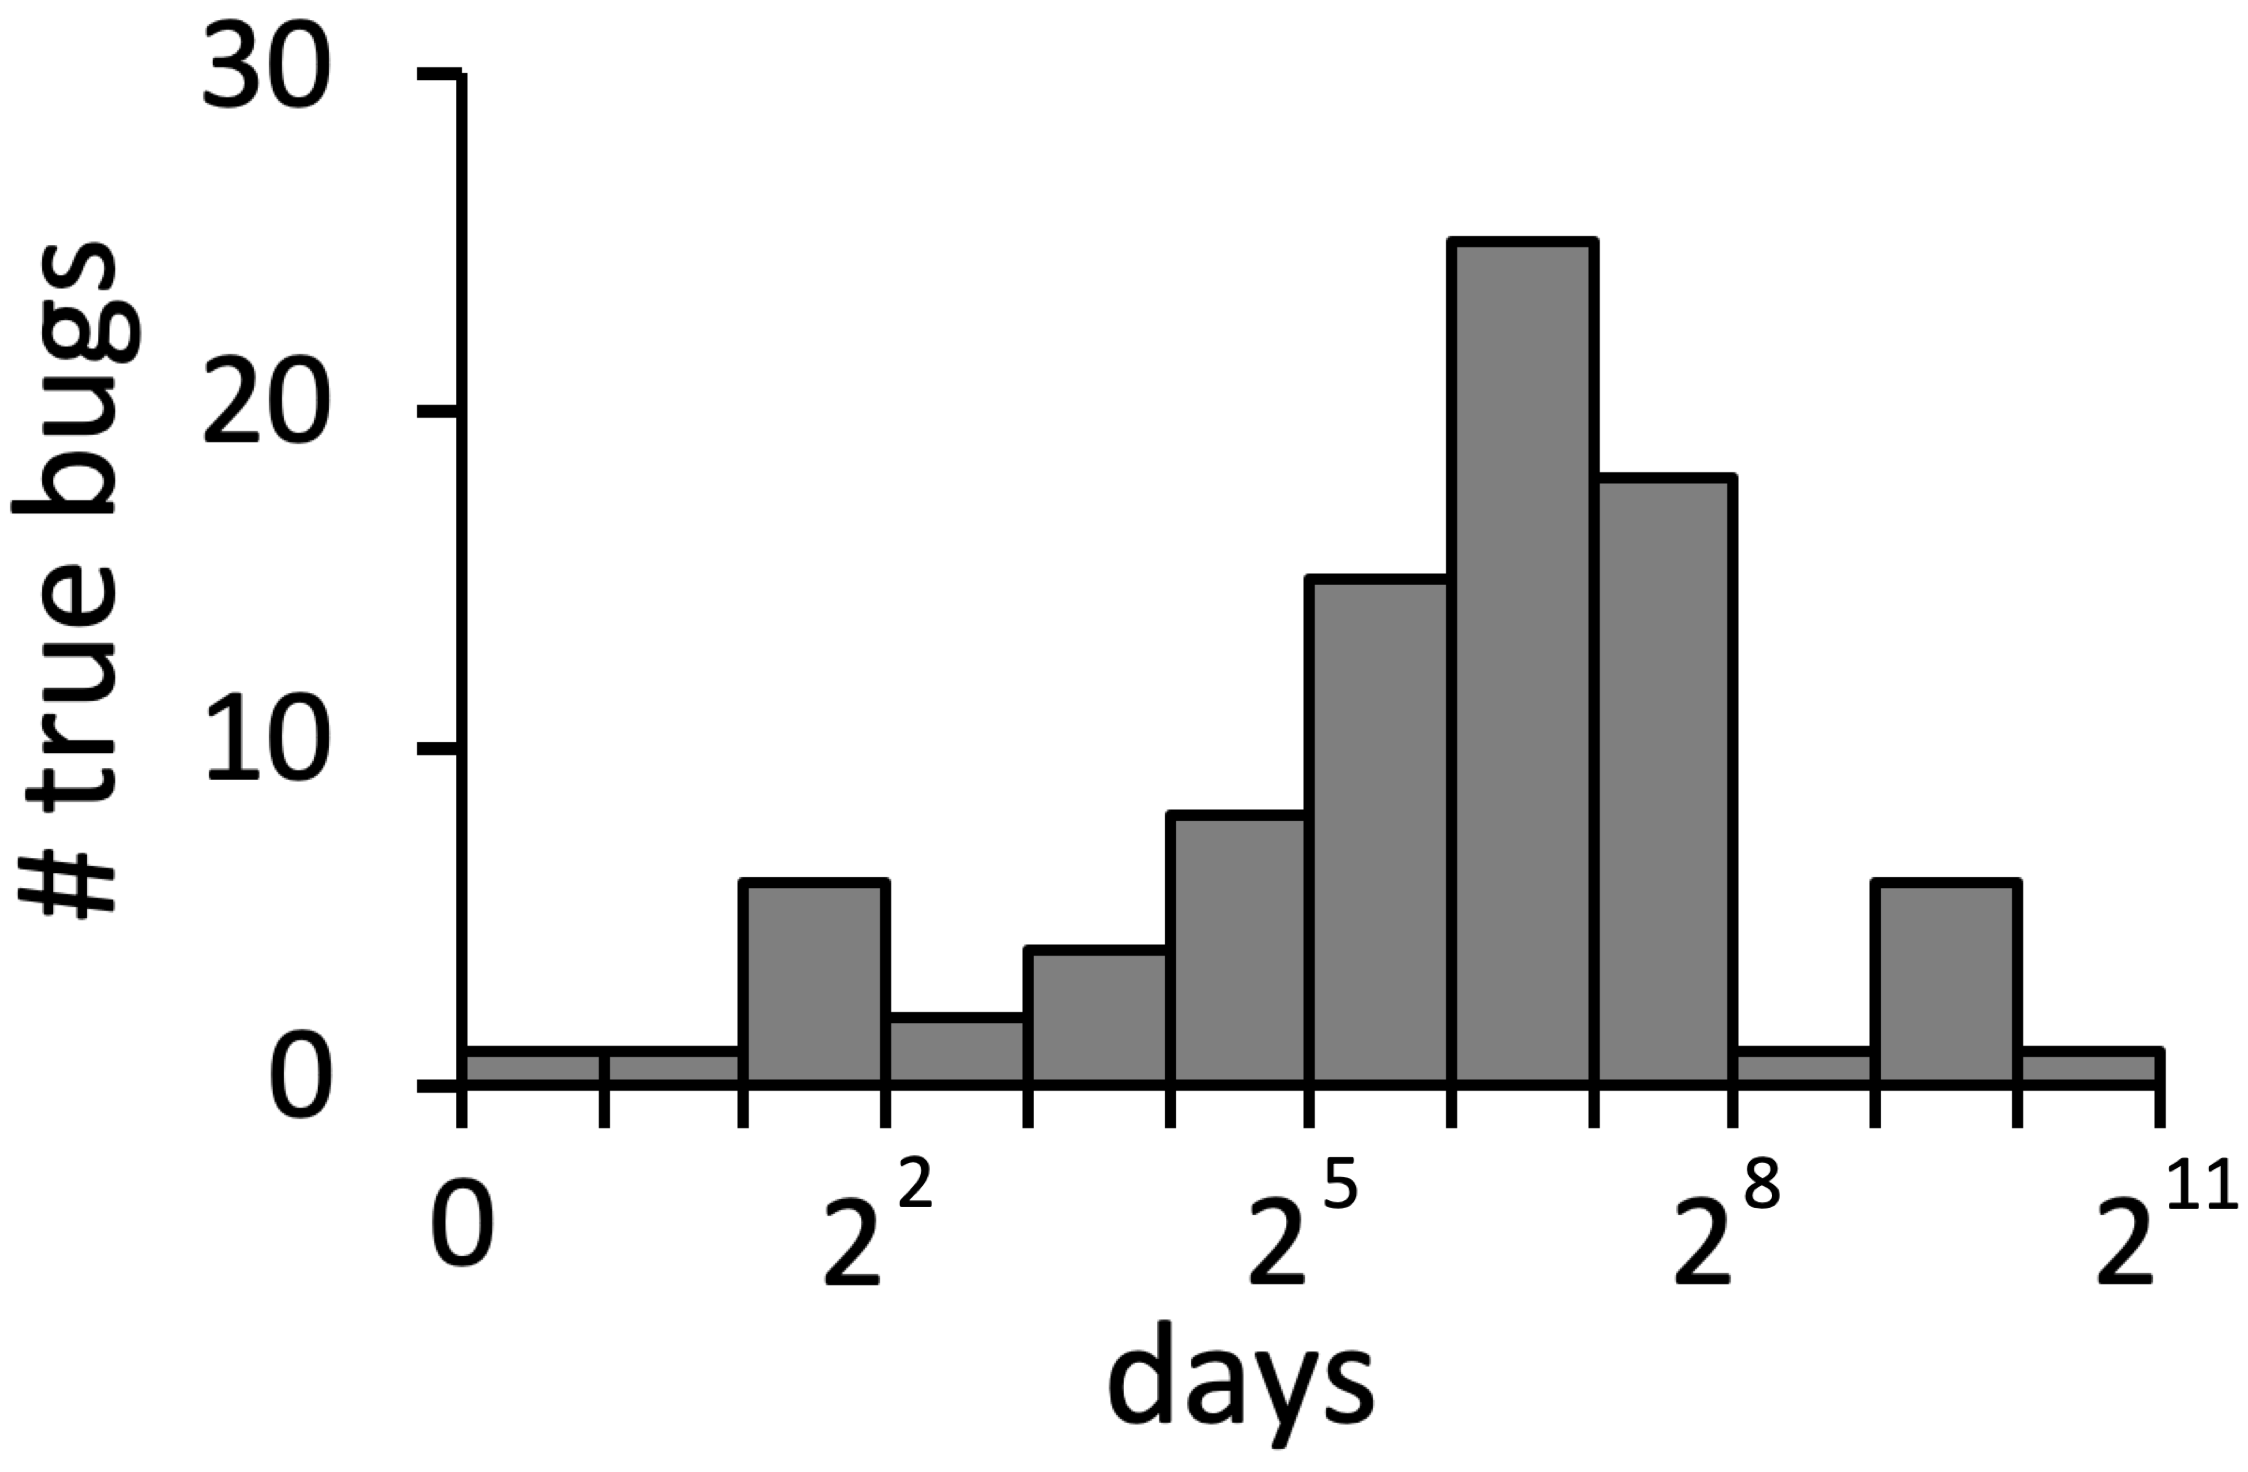
\includegraphics[width=\textwidth]{img/ttl-count}
    \caption{The histogram by TTL.}
  \end{subfigure}
  \caption{Time to Live (TTL) of true bugs.}
  \vspace*{-1.5em}
  \label{fig:ttl}
\end{figure}

We measured the analysis precision based on the number of true bugs in
type-related specification bugs detected by $\tool$.  As described in the
\stextsf{refine} column of Table~\ref{table:precision}, the analysis precision
is \inred{51.7}\% because it detected \inred{190} type-related bugs and
\inred{89} bugs are true bugs among them.  The reference checker detected the
largest number of bugs with \inred{51.7}\% precision; it found \inred{12} true
reference bugs for \inred{32} unknown variables (\stextsf{UnknownVar}) and
\inred{32} already defined variables (\stextsf{DuplicatedVar}). The arity
checker and the assertion checker found \inred{12} missing parameters
(\stextsf{MissParam}) with \inred{90.2}\% precision and \inred{12} assertion
failures (\stextsf{Assertion}) with \inred{90.2}\% precision, respectively.
Finally, the operand checker detected two different kinds of wrong typed operand
bugs: \inred{12} non-numeric operand bugs (\stextsf{NoNumber}) for numeric
operators with \inred{12.3}\% precision and \inred{12} unchecked abrupt
completion bugs (\stextsf{Abrupt}) with \inred{12.3}\% precision.

Moreover, we extended $\tool$ to automatically extract more statistics of
detected true bugs.  \inred{First, we checked that true bugs are created or
resolved by whom as described in Table~\ref{table:author}.  Among \inred{89}
true bugs, we cannot automatically know who created \inred{20} inherited bugs
created before 2018.  For remaining \inred{20} bugs, only \inred{20} bugs are
created by members of the Ecma Technical Committee 39 (TC39) but others
(\inred{20} bugs) are created by outside contributors not committee members.
On the other hand, most of them (\inred{20} bugs) are resolved by the committee
members but only \inred{20} bugs are resolved by non-committee contributors.
Other \inred{14} bugs are newly found and we will explain their details in
Section~\ref{sec:new-bug}.}  Another statistic of true bugs is Time to Live
(TTL) that denotes how many days specification bugs existed.
Figure~\ref{fig:ttl} describes TTL of true bugs; the left chart depicts the
period of existing bugs sorted by their creation time, and the right chart
depicts the histogram of TTL in a logarithmic scale.  The average TTL of true
bugs is \inred{300.0} days although we assume that \inred{20} inherited bugs are
created in January 1, 2018.  The maximum length of TTL is \inred{1,000} and this
bug is created before 2018 but not yet resolved in the latest version.  We
manually investigated the creation time of this bug, and we discovered that it
was created at the initial commit of the open development process in September
22, 2015.  It means that the bug actually existed for \inred{3,000} days.


\subsection{Effectiveness of Refinement}\label{sec:effect-refine}

We showed that the condition-based refinement for type analysis of ECMAScript
effectively increased analysis precision without significant performance
degradation. \todo

\begin{figure}
  \centering
  \begin{subfigure}[b]{0.24\textwidth}
    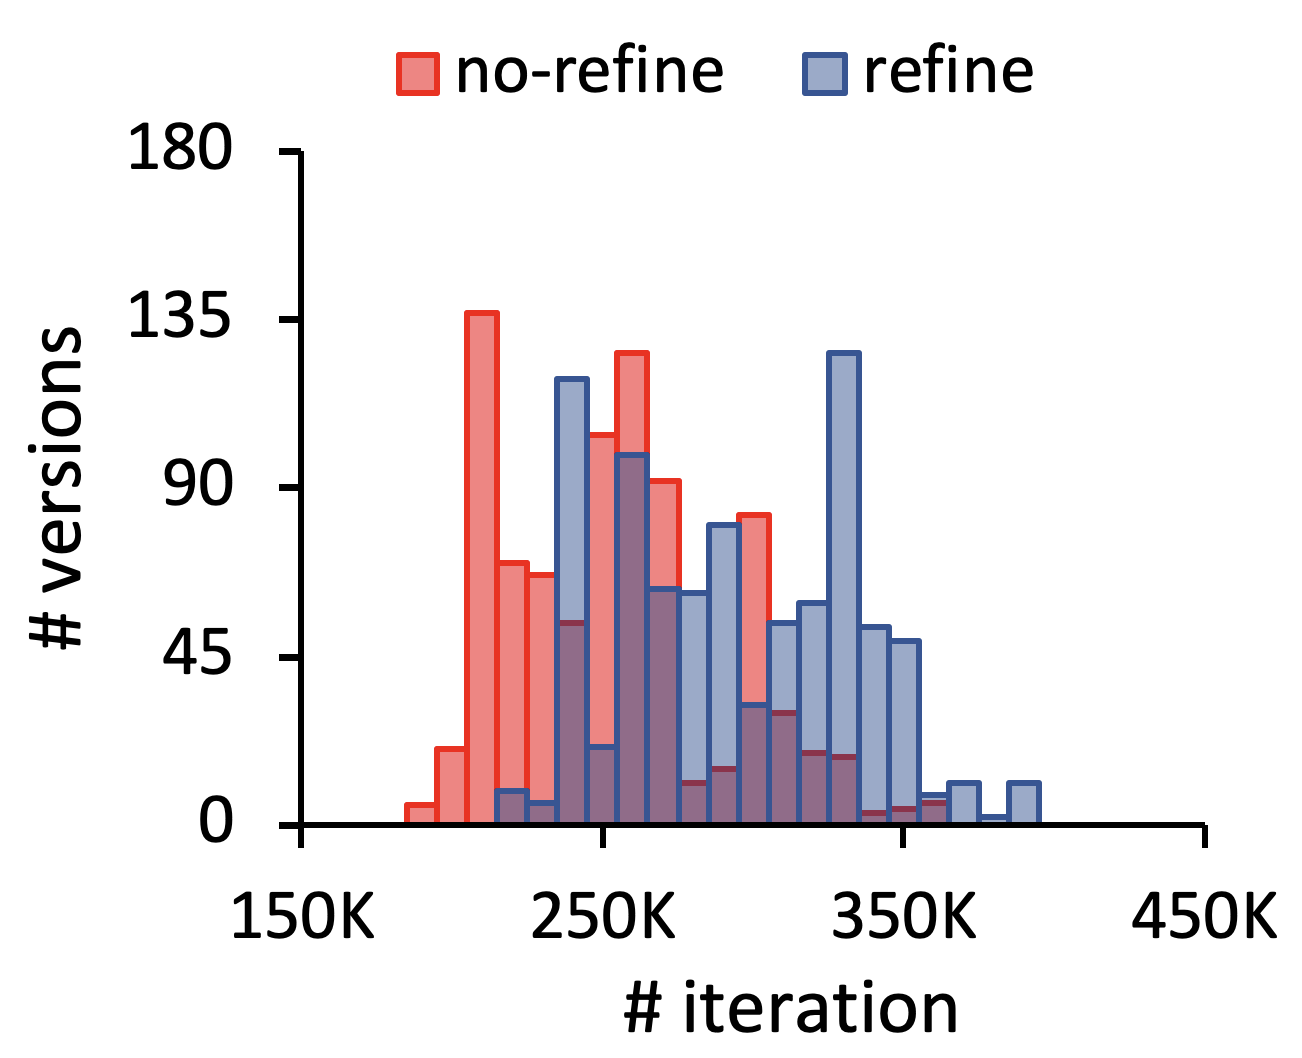
\includegraphics[width=\textwidth]{img/compare-iter}
    \caption{The number of iterations.}
  \end{subfigure}
  \begin{subfigure}[b]{0.24\textwidth}
    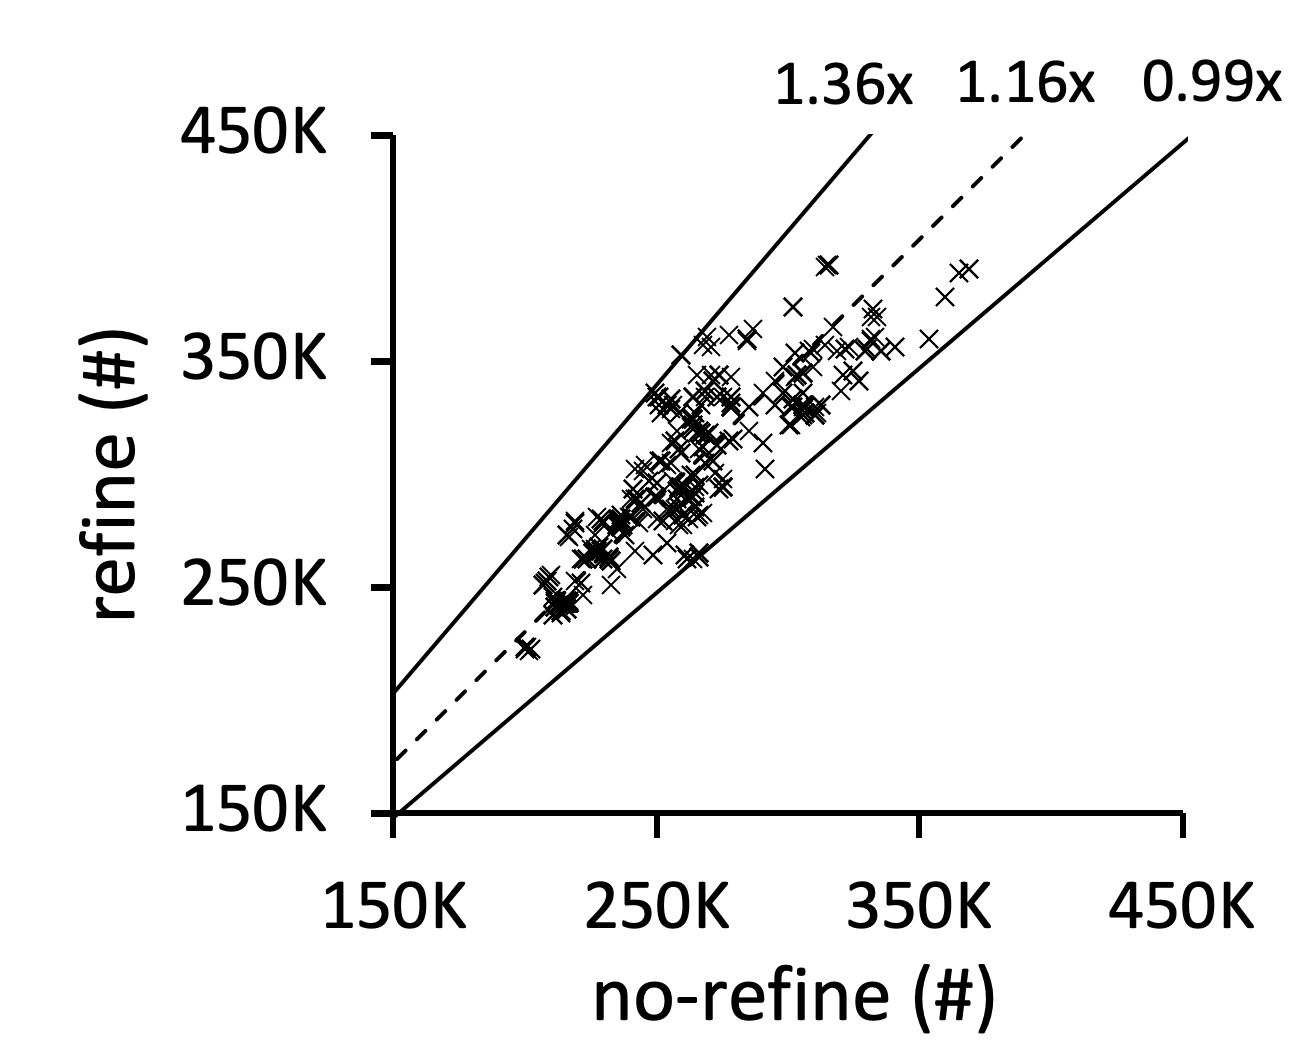
\includegraphics[width=\textwidth]{img/ratio-iter}
    \caption{The ratio of iterations.}
  \end{subfigure}
  \begin{subfigure}[b]{0.24\textwidth}
    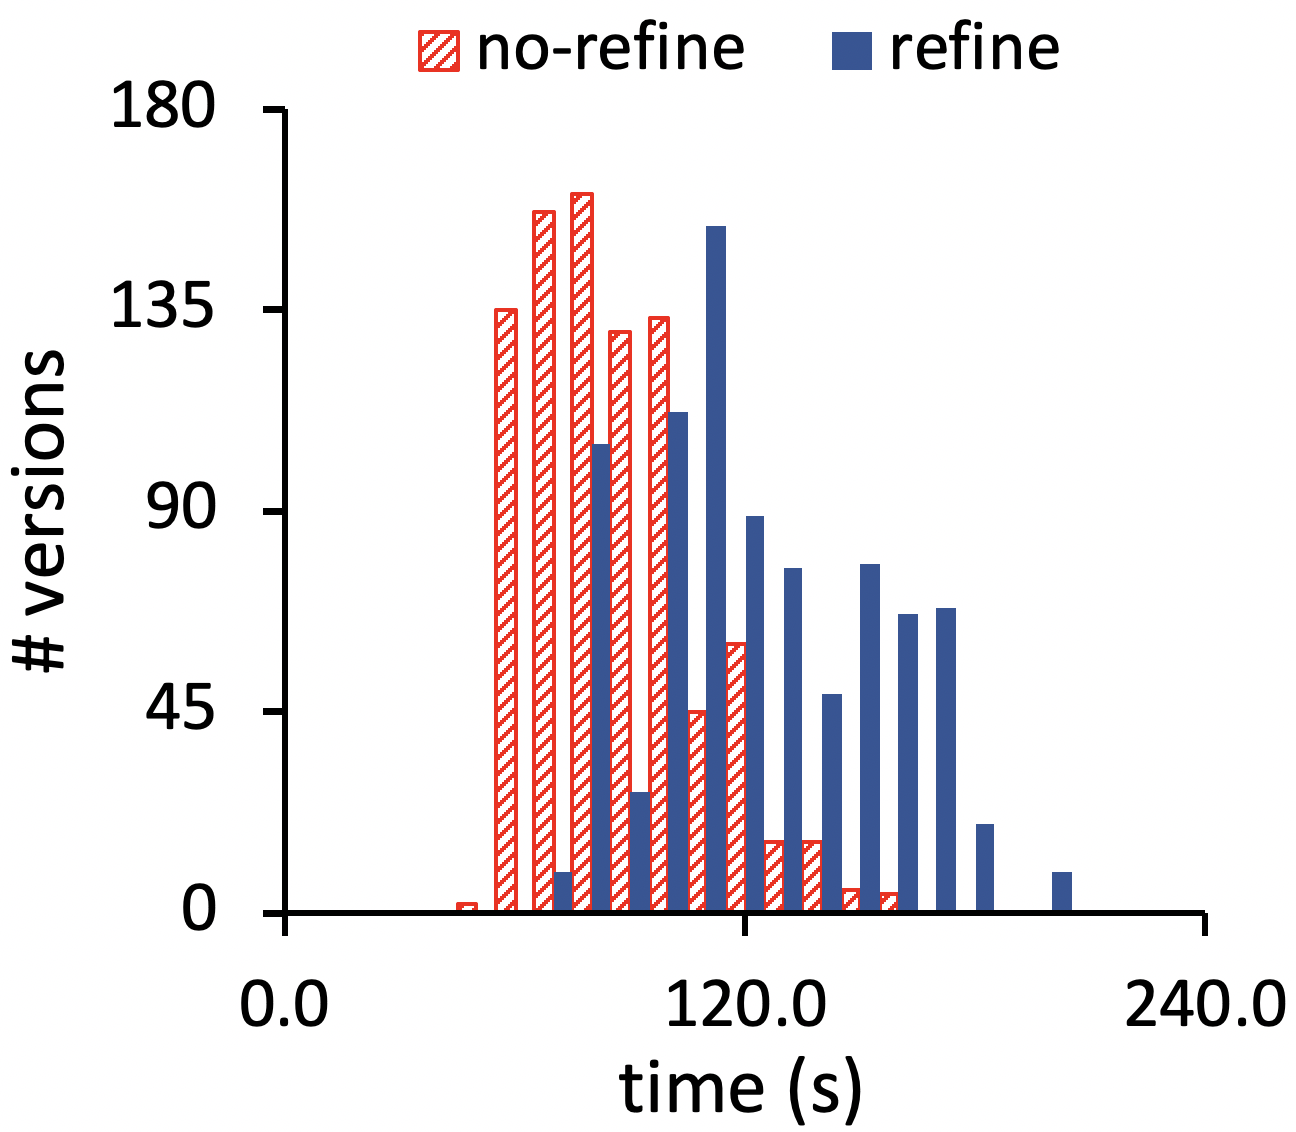
\includegraphics[width=\textwidth]{img/compare-time}
    \caption{The analysis time.}
  \end{subfigure}
  \begin{subfigure}[b]{0.24\textwidth}
    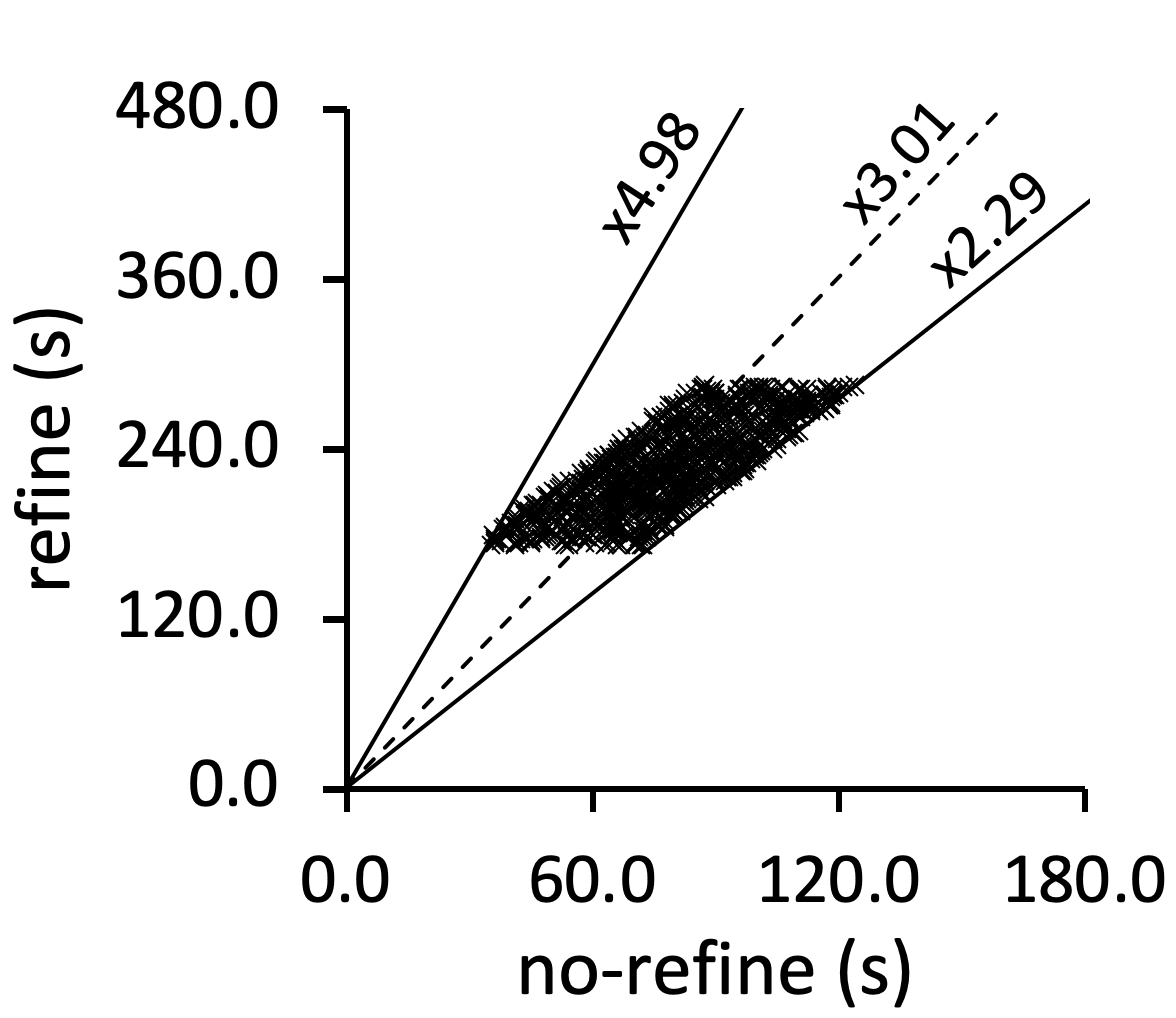
\includegraphics[width=\textwidth]{img/ratio-time}
    \caption{The ratio of analysis time.}
  \end{subfigure}
  \caption{The comparison of iterations and analysis time without refinement
  (\stextsf{no-refine}) and those with refinement (\stextsf{refine}).}
  \label{fig:performance-comp}
  \vspace*{-1.5em}
\end{figure}


\subsection{Detection of New Bugs}\label{sec:new-bug}

\begin{table*}
  \centering
  \caption{Type-related specification bugs newly detected by $\tool$ in the
  official draft of ECMAScript 2021 (ES12).}
  \label{table:new-bug}
  \resizebox{\textwidth}{!}{%
  \begin{tabular}{@{}c@{~}?c|@{~}c@{~}|l|c|@{~}c@{~}|@{~}c@{~}|@{~}r@{}}
    \multicolumn{1}{@{}c?}{\textbf{Name}} &
    \multicolumn{1}{c}{\textbf{Feature}} &
    \multicolumn{1}{@{}c@{~}}{\textbf{\#}} &
    \multicolumn{1}{c}{\textbf{Description}} &
    \multicolumn{1}{@{~}c@{~}}{\textbf{Checker}} &
    \multicolumn{1}{@{}c}{\textbf{Created}} &
    \multicolumn{1}{@{}c}{\textbf{Resolved}} &
    \multicolumn{1}{@{}c@{~}}{\textbf{TTL}}\\\specialrule{.1em}{.0em}{.0em}

    ES12-1 &
    Switch &
    3 &
    \makecell[l]{
        Variables \code{hasDuplicates} and \code{hasUndefinedLabels} are already \\
        defined in algorithms for \jscode{case} blocks of \jscode{switch}
        statements.
    } &
    \stextsf{Reference} &
    \inred{2015-01-01} &
    \inred{2015-01-01} &
    \inred{1,999} days\\\hline

    ES12-2 &
    Try &
    3 &
    \makecell[l]{
        Variables \code{hasDuplicates} and \code{hasUndefinedLabels} are already \\
        defined in algorithms for \jscode{try} statements.
    } &
    \stextsf{Reference} &
    \inred{2015-01-01} &
    \inred{2015-01-01} &
    \inred{1,999} days\\\hline

    ES12-3 &
    Arguments &
    1 &
    \makecell[l]{
        A variable \code{index} is already defined in
        \textbf{CreateMappedArgumentsObject}.
    } &
    \stextsf{Reference} &
    \inred{2015-01-01} &
    \inred{2015-01-01} &
    \inred{1,999} days\\\hline

    ES12-4 &
    Array &
    2 &
    \makecell[l]{
        A variable \code{succeeded} is already defined in algorithms for
        \jscode{Array} objects.
    } &
    \stextsf{Reference} &
    \inred{2015-01-01} &
    \inred{2015-01-01} &
    \inred{1,999} days\\\hline

    ES12-5 &
    Class &
    1 &
    \makecell[l]{
        A variable \code{ClassHeritage} is not defined in \textbf{Contains}
        \\ for tails of \jscode{class} declarations.
    } &
    \stextsf{Reference} &
    \inred{2015-01-01} &
    \inred{2015-01-01} &
    \inred{1,999} days\\\hline

    ES12-6 &
    Branch &
    1 &
    \makecell[l]{
        A variable \code{Statement} is not defined in \textbf{EarlyErrors} for
        \jscode{if} statement.
    } &
    \stextsf{Reference} &
    \inred{2015-01-01} &
    \inred{2015-01-01} &
    \inred{1,999} days\\\hline

    ES12-7 &
    Async &
    1 &
    \makecell[l]{
        A variable \code{value} is already defined in \textbf{Evaluation} for
        \jscode{yield} expressions.
    } &
    \stextsf{Reference} &
    \inred{2015-01-01} &
    \inred{2015-01-01} &
    \inred{1,999} days\\\hline

    ES12-8 &
    Arguments &
    2 &
    \makecell[l]{
        Abrupt completions are used in \textbf{DefineOwnProperty} and
        \textbf{GetOwnProperty} \\ for \jscode{arguments} objects without any
        checks.
    } &
    \stextsf{Operand} &
    \inred{2015-01-01} &
    \inred{2015-01-01} &
    \inred{1,999} days\\
  \end{tabular}
  }
  \vspace*{-1.5em}
\end{table*}
